% ---------------------------------------------------------------
% Section: Conclusions & Next Steps
% ---------------------------------------------------------------

\section[Conclusions]{Conclusions \& Next Steps}

\begin{frame}{Current Status}
\begin{columns}
\begin{column}{0.5\textwidth}
\begin{myalert}[Keep]
\small LodeSTAR detection + reference-calibrated correction is promising, but transfer must be validated per run.
\end{myalert}
\smallskip
\begin{mynote}
\footnotesize Correct claim: improves LodeSTAR positions relative to reference detections when validation passes.\\
Incorrect claim: recovers ground truth.
\end{mynote}
\end{column}
\begin{column}{0.5\textwidth}
\begin{myalert}[Do not over-invest]
\small Plain ABP and gap filling are useful diagnostics, but neither is the main solution for imperfect detections.
\end{myalert}
\smallskip
\begin{mynote}
\footnotesize ABP is unstable under interaction filtering; BiLSTM changes too few production rows.
\end{mynote}
\end{column}
\end{columns}
\end{frame}

\begin{frame}{Next Validation Gate}
\begin{columns}
\begin{column}{0.52\textwidth}
\begin{figure}
    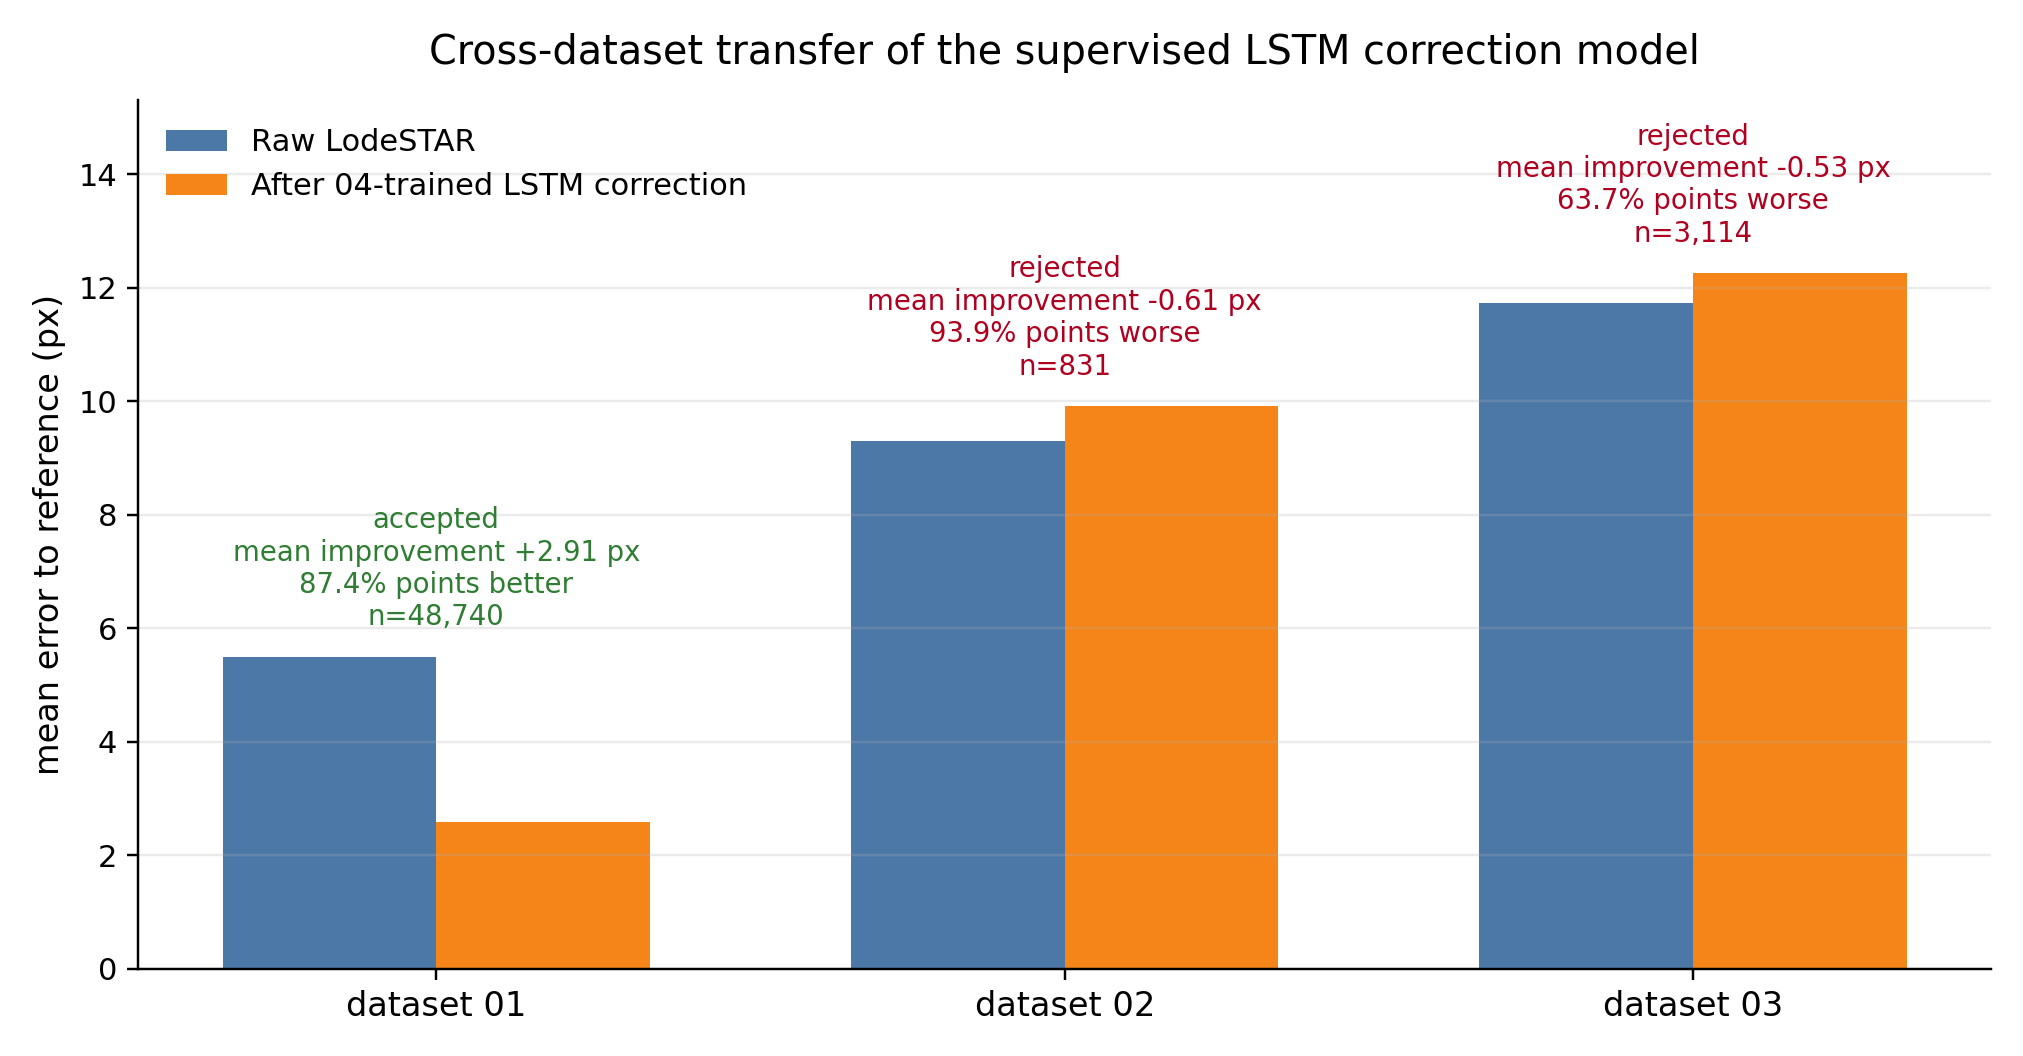
\includegraphics[width=\textwidth]{imglib/progress_update/supervised_transfer_01_02_03_bar.png}
\end{figure}
\end{column}
\begin{column}{0.48\textwidth}
\begin{enumerate}\small
    \item Accept \texttt{04}$\rightarrow$\texttt{01} as a positive transfer case
    \item Reject \texttt{04}$\rightarrow$\texttt{02}/\texttt{03} for final export
    \item Train a multi-run or run-specific corrector
    \item Export corrected tracks only after a held-out reference check
\end{enumerate}
\end{column}
\end{columns}
\end{frame}
